\setcounter{section}{0}
\section{Hình thành kiến thức mới}
\subsection{Sử dụng nhiên liệu hóa thạch}
Nhiên liệu hóa thạch như than đá, dầu mỏ, khí thiên nhiên, $\ldots$ được hình thành nhờ sự phân hủy xác động vât, thực vật và quá trình biến đổi của địa chất trong hàng triệu năm.

Than đá là nguồn năng lượng chủ yếu trong các ngành nhiệt điện, xi măng, luyện kim và phân bón. Than đá cháy trong không khí tỏa ra nhiều nhiệt, nhưng thải ra nhiều loại khí độc như SO$_2$, CO, NO$_2$, $\ldots$ và bụi mịn gây hại cho phổi, tim và hệ thần kinh của con người.
\subsection{Sử dụng năng lượng tái tạo}
%\begin{center}
%	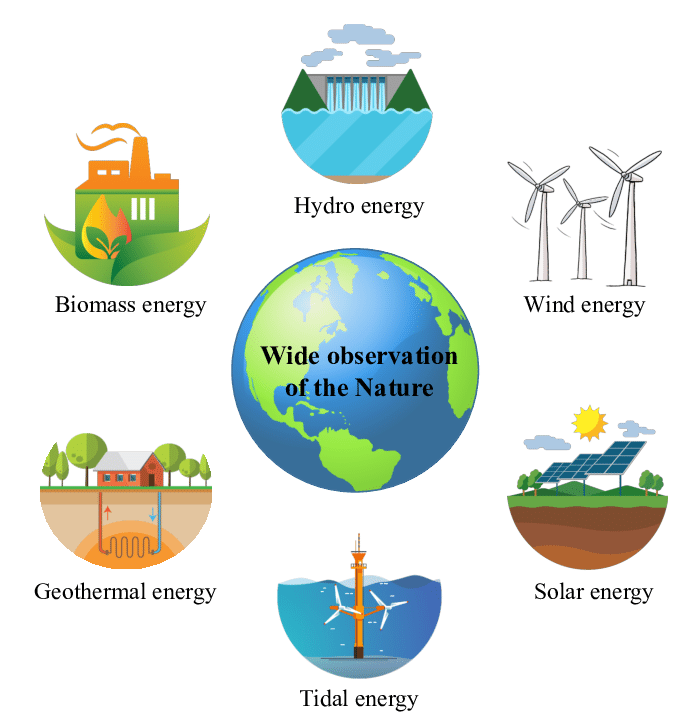
\includegraphics[width=\textwidth]{../figs/G10-036-1.png}
%\end{center}
Năng lượng tái tạo là dạng năng lượng được cung cấp bởi những nguồn nguyên liệu có sẵn trong tự nhiên và không bao giờ cạn kiệt hoặc có thời gian sử dụng rất lớn như năng lượng Mặt Trời, gió, nước, thủy triều, địa nhiệt, sinh khối, $\ldots$.

Năng lượng tái tạo có vai trò quan trọng trong sự phát triển kinh tế, xã hội và bảo vệ môi trường để đảm bảo phát triển bề vững. Cụ thể là:
\begin{itemize}
	\item Năng lượng tái tạo có trữ lượng vô hạn, có tiềm năng thay thế các nguồn năng lượng hữu hạn như năng lượng hóa thạch, góp phần tránh được các hậu quả có hại đến môi trường.
	\item Việc phát triển năng lượng tái tạo được xem là bước đi tiên phong cho việc giảm khí thải gây ra hiệu ứng nhà kính.
	\item Việc sử dụng năng lượng tái tạo góp phần tăng cường nguồn cung trong nước, giảm thiểu sự phụ thuộc vào nguồn năng lượng nhập khẩu nước ngoài, đảm bảo an ninh năng lượng quốc gia.
\end{itemize}

Một số công nghệ cơ bản để thu được năng lượng tái tạo:
\begin{itemize}
	\item Điện Mặt Trời: sử dụng pin Mặt Trời biến đổi năng lượng ánh sáng Mặt Trời thành điện năng. Quá trình chuyển hóa năng lượng này xảy ra theo các giai đoạn sau: ánh sáng Mặt Trời chiếu tới làm xuất hiện các hạt mang điện trong tấm bán dẫn, dưới tác dụng của một hiệu điện thế, các hạt mang điện này chuyển động có hướng để tạo thành dòng điện.
	\item Nhiệt Mặt Trời: Quang năng từ bức xạ Mặt Trời được chuyển hóa thành nhiệt năng sử dụng trong một số thiết bị như: bếp, máy nước nóng sử dụng năng lượng Mặt Trời.
	\item Năng lượng gió: Năng lượng gió có thể chuyển thành cơ năng trong cối xay gió hoặc sử dụng gián tiếp thông qua các thiết bị chuyển đổi như tuabin gió để chuyển thành năng lượng điện.
	\item Năng lượng sinh khối: Đê chuyển năng lượng sinh khối thành điện năng, ta có thể sử dụng một số phương pháp như: đốt trực tiếp và sử dụng lò hơi; đôt liên kết; nhiệt phân.
	\item Năng lượng nước: Thế năng trọng trường của nước được tích lũy tại các đập thủy điện ở trên cao. Sau khi nước được xả ra và chảy xuống dưới, động năng của nó làm quay tuabin và phát ra điện.
	\item Năng lượng đại dương: Bao gồm năng lượng thủy triều, năng lượng sóng, năng lượng nhiệt đại dương.
	\item Năng lượng địa nhiệt: từ các nguồn đá nóng, nước nóng ngầm dưới đất như núi lửa, suối nước nóng, hồ nước nóng.
\end{itemize}
\subsection{Sử dụng năng lượng ở Việt Nam hiện nay}
Trong những năm qua, Việt Nam là nền kinh tế năng động, phát triển khá nhanh. Ngành năng lượng đóng vai trò then chốt trong việc thúc đẩy phát triển kinh tế - xã hội.

Hiện nay, năng lượng thủy điện đã gần như khai thác hết, trữ lượng than đá cũng đang cạn dần. Việc sử dụng nhiều năng lượng hóa thạch cũng gây ô nhiễm môi trường.

Việc sử dụng năng lượng không hiệu quả gây nhiều hiện tượng khí hậu cực đoan như nắng nóng khắc nghiệt, cháy rừng, lũ lụt, bão lũ đã ảnh hưởng đến hàng triệu người, đồng thời gây ra những hiểm họa đối với sức khỏe, an ninh và phát triển kinh tế. Việt Nam là nước chịu thiệt hại nặng nề nhất của biến đổi khí hậu. So sánh với một số nước đang phát triển chịu tác động của biến đổi khí hậu thì Việt Nam là quốc gia chịu thiệt hại tính trên GDP cao nhất.

Trong tương lai, Việt Nam cần khai thác hợp lí, hiệu quả và sử dụng nguồn năng lượng hiện có, mở rộng khai thác các nguồn năng lượng tái tạo, thân thiện với môi trường.
\section{Mở rộng}
\subsection{Sử dụng năng lượng hiệu quả trong đời sống và sản xuất}
Sử dụng năng lượng hiệu quả là mục tiêu của những nỗ lực nhằm giảm năng lượng cần thiết cung cấp cho sản xuất và dịch vụ.

Việc sử dụng điện sinh hoạt quá mức như máy điều hòa, tủ lạnh tiêu tốn nhiều năng lượng. Các máy làm lạnh là thiết bị dùng để chuyển nhiệt lượng từ nơi lạnh sang nơi nóng bằng cách sử dụng điện năng để nén và dãn nở khí làm nhiệt độ của nó tăng lên và truyền ra môi trường.

Điều hòa nhiệt độ là thiết bị sử dụng điện năng giúp hạ nhiệt độ hoặc tăng nhiệt độ trong phòng. Việt thiết kế công trình, lắp đặt và sử dụng điều hòa hợp lí sẽ giúp tiết kiệm điện năng.

Tủ lạnh là một thiết bị làm mát, gồm ngăn cách nhiệt và hệ thống để truyền nhiệt từ nó ra môi trường bên ngoài. Tủ lạnh có thể duy trì nhiệt độ trong ngăn cách nhiệt ở nhiệt độ lạnh nhất định.

Để sử dụng tủ lạnh tiết kiệm điện cần bố trí tủ ở nơi thoáng mát và sử dụng hợp lí.

Bình nước nóng là một thiết bị điện gia dụng cung cấp nguồn nước nóng dựa vào việc chuyển điện năng thành nhiệt năng khi cho dòng điện chạy qua dây dẫn. Lựa chọn và sử dụng bình nước nóng không hợp lí sẽ tiêu hao nhiều điện năng.

Xe máy, ô tô, máy phát điện, $\ldots$ sử dụng nhiên liệu đốt trong xi lanh của động cơ làm hệ thống động cơ nóng lên. Hệ thống làm mát của động cơ rất quan trọng. Nếu hệ thống làm mát bám bụi bẩn, không được bổ sung nước làm mát đầy đủ sẽ ảnh hưởng đến quá trình thải nhiệt ra môi trường, khiến nhiệt độ buồng máy tăng cao. Hiệu suất động cơ sẽ thấp và tốn nhiên liệu. Vì vậy, nên vệ sinh sạch sẽ, bổ sung nước làm mát đầy đủ cho một số động cơ.
\section{Tự luận}
\setcounter{section}{0}

\begin{enumerate}[label=\bfseries Câu \arabic*:]
	\item \mkstar{2}
	
	{
		Việt Nam đang khai thác các nguồn năng lượng nào? Tiềm năng khai thác nguồn năng lượng của Việt Nam như thế nào?
	}
	
	\hideall{
		
		Việt Nam đang khai thác các nguồn năng lượng:
		
		- Than: Tổng trữ lượng than Việt Nam được xác định khoảng 2,2 tỷ tấn, chủ yếu ở bể Đông Bắc, có thể khai thác trong khoảng 40 năm nữa (với mức khai thác như hiện tại).
		
		Theo số liệu tính toán, khai thác than thương phẩm sẽ đạt khoảng 53 - 54,8 triệu tấn vào giai đoạn 2030 - 2035. 
		
		- Dầu khí: trữ lượng khí tại mỏ Kèn Bầu được phát hiện khá lớn (ước tính có thể tới 200 - 250 tỷ m$^3$), nhưng hiện chưa được khẳng định chắc chắn về trữ lượng.
		
		- Nước: tiềm năng phát triển thủy điện của Việt Nam đã gần cạn kiệt.
		
		- Mặt trời: Ước tính tổng tiềm năng kỹ thuật điện mặt trời của Việt Nam như sau: Điện mặt trời (quy mô lớn trên mặt đất) khoảng 309 GW; điện mặt trời (trên mặt nước) khoảng 77 GW và điện mặt trời (trên mái nhà) khoảng 48 GW.
		
		- Gió: Nằm trong khu vực cận nhiệt đới gió mùa với bờ biển dài, gió tại Biển Đông khá mạnh và thay đổi theo mùa, Việt Nam có thuận lợi để phát triển năng lượng gió. Tổng tiềm năng kỹ thuật điện gió (trên bờ) của nước ta khoảng 217 GW và tổng tiềm năng kỹ thuật điện gió (ngoài khơi) khoảng 160 GW.
		
		- Địa nhiệt: Điện địa nhiệt có tiềm năng kỹ thuật khoảng 0,7 GW, phần lớn ở miền Bắc (0,4 GW). 
		
		
	}
	
	\item \mkstar{2}
	

	{
		Tại sao thông qua chỉ số tiêu dùng năng lượng bình quân theo đầu người, có thể phán đoán trình độ phát triển kinh tế, kĩ thuật và văn hóa của một quốc gia?
	}
	
	\hideall
	{
		Do nền sản xuất hiện đại chỉ có thể phát triển nhờ ngành năng lượng. 
	}
	\item \mkstar{2}
	
	
	{
		Nêu những ưu điểm và khuyết điểm khi phát triển năng lượng tái tạo tại Việt Nam.
	}
	
	\hideall
	{
		\textbf{Ưu điểm:}
		
		Năng lượng tái tạo là nguồn năng lượng sạch, thân thiện với môi trường, ít gây ô nhiễm. Nhiều ứng dụng từ nguồn năng lượng này rất hữu ích, giúp tiết kiệm điện năng cho các hộ gia đình, nhà máy, xí nghiệp.
		
		Đó là nguồn năng lượng lớn không sợ cạn kiệt, có thể sử dụng cho nhiều nhu cầu, và địa điểm khác nhau.
		
		Do nó là nguồn năng lượng từ thiên nhiên nên chi phí nhiên liệu và bảo dưỡng thấp, cũng như độ bền cao hơn gấp nhiều lần.
		
		\textbf{Nhược điểm:}
		
		Điểm trừ của năng lượng tái tạo là chi phí đầu tư ban đầu thường cao, hiệu suất hoạt động có thể bị ảnh hưởng bởi các yếu tố thời tiết, thiên nhiên. Năng lượng tái tạo rất khó khăn để sản xuất một lượng điện lớn.
	}
	\item \mkstar{2}
	
	
	{
		Trình bày tác hại của việc xây dựng đập thủy điện đến diện tích cây xanh.
	}
	
	\hideall
	{
		
		Trong quá trình xây dựng thủy điện, hàng loạt diện tích rừng đã bị xâm chiếm khiến cho môi trường mất lớp cây xanh sản xuất oxi, giảm thiểu khí cacbondioxit. Không chỉ thế, mất đi cây xanh khiến cho môi trường mất đi lớp màn bảo vệ trước bụi, đất li ti trong không khí. Đây là một trong những nguyên nhân khiến không khí ngày càng trở nên ô nhiễm và gây hại cho sức khỏe của con người.
		
		Các nhà khoa học cho rằng, nguyên nhân của lũ quét, sạt lở đất có liên quan tới độ dốc lớn về địa hình của khu vực miền núi đi liền với diễn biến mưa lớn phức tạp và sự suy giảm độ che phủ rừng, thảm thực vật. Đặc biệt là các tác động của con người, trong đó trọng tâm là chặt phá rừng và xây dựng các hồ chứa, đập thủy điện.
		
		Rừng bị mất đi quá nhiều là nguyên nhân làm cho lũ lụt ngày càng gia tăng. Mưa lớn ở thượng nguồn, nước chảy nhanh xuống không có lớp rừng để giảm sốc tạo thành lũ gây thiệt hại nặng nề. Lũ lụt xảy ra thường xuyên và tàn khốc hơn còn do các nhà máy thủy điện xả lũ vì nguy cơ vỡ đập trong mùa mưa bão.
		
	}
	
	\item \mkstar{2}
	
	{
		Hãy nêu ra các tác động gây biến đổi khí hậu bởi các nhà máy nhiệt điện, nhà máy thủy điện, phương tiện giao thông.
	}
	
	\hideall{
		
		Các nhà máy thủy điện xây dựng ở thượng nguồn các con sông làm ảnh hưởng đến dòng nước ở hạ lưu gây ra biến đổi khí hậu, hạn hán, xâm nhập mặn.
		
		Sự biến đổi của dòng chảy các con sông như sông Mê Kông gây hạn hán ở Đồng bằng Sông Cửu Long làm mất mùa, cùng với thiếu điện làm sản xuất, kinh doanh bị tổn thất lớn.
		
		Các nhà máy nhiệt điện chạy bằng nhiên liệu hóa thạch thải nhiều khói bụi, khí CO$_2$ làm ảnh hưởng đến bầu khí quyển. Các phương tiện giao thông sử dụng xăng, dầu góp phần gây ra sự nóng lên của toàn cầu.
	}
	
	\item \mkstar{2}
	
	
	{
		Hãy nêu một số biện pháp tiết kiệm năng lượng khi sử dụng các thiết bị điện trong gia đình em.
	}
	
	\hideall
	{
		1. Không nên để thiết bị điện ở trạng thái chờ.
		
		2. Sử dụng các thiết bị có nhãn xác nhận là sản phẩm tiết kiệm điện.
		
		3. Lắp các thiết bị cảm biến chuyển động để tránh lãng phí điện.
		
		4. Thay các bóng đèn chiếu sáng thường bằng bóng đèn Led.
		
		5. Sử dụng các sản phẩm công nghệ Inverter.
		
		
		6. Sử dụng các thiết bị hẹn giờ để bật/tắt thiết bị điện gia dụng.
		
		7. Tận dụng tối đa nguồn ánh sáng và nguồn gió từ môi trường bên ngoài.
		
		8. Sơn tường và sử dụng vật dụng trong nhà có tông màu sáng.
		
		9. Thay đổi thói quen sử dụng các thiết bị điện trong gia đình.
		
		10. Sử dụng nguồn điện năng lượng mặt trời.
	}
	\item \mkstar{2}
	
	
	{
		Tại sao nước thải mỏ gây ô nhiễm nguồn nước?
	}
	
	\hideall
	{
		Trong những năm gần đây, hoạt động khai thác và chế biến khoáng sản (HĐKS) phát triển một cách ồ ạt, gây những tác động tiêu cực tới môi trường, đặc biệt gây ô nhiễm và suy thoái nguồn nước sản xuất nông nghiệp. Trong HĐKS, nước được sử dụng với khối lượng lớn cho hầu hết công đoạn sản xuất. Quá trình sản xuất, tháo khô mỏ, đổ thải, v.v… đã gây những tác động tiêu cực tới nguồn nước sản xuất nông nghiệp ở khu vực xung quanh khai trường như thay đổi địa hình, hệ thống nước mặt, điều kiện tàng trữ và thoát nước (tác động cơ học) làm thay đổi tính chất vật lý, thành phần hóa học của nước (tác động hóa học).
		
		\textbf{Ảnh hưởng của những tác động cơ học của HĐKS tới nguồn nước}
		
		Quá trình đào xới, vận chuyển đất đá và quặng làm địa hình khu khai trường bị hạ thấp, ngược lại, quá trình đổ chất thải rắn làm địa hình bãi thải được tâng cao. Những thay đổi này sẽ dẫn đến những biến đổi về điều kiện thủy văn, các yếu tố của dòng chảy trong khu mỏ như: Thay đổi khả năng thu, thoát nước, hướng và vận tốc dòng chảy mặt, chế độ thủy văn của các dòng chảy như mực nước, lưu lượng, v.v….
		
		Sự tích tụ chất thải rắn do tuyển rửa quặng trong các lòng hồ, kênh mương tưới tiêu có thể làm thay đổi lưu lượng dòng chảy, dung tích chứa nước, biến đổi chất lượng nguồn nước và làm suy giảm công năng của các công trình thuỷ lợi nằm liền kề với các khu khai thác mỏ.
		
		Khi tiến hành các HĐKS sẽ hình thành các moong sâu đến hàng trăm mét, là nơi tập trung nước cục bộ. Ngược lại, để đảm bảo hoạt động của mỏ, phải thường xuyên bơm tháo khô nước ở đáy moong, hầm lò, hình thành các phễu hạ thấp mực nước dưới đất với độ sâu mực từ vài chục đến hàng trăm mét và bán kính phễu hàng trăm mét. Điều đó dẫn đến tháo khô các công trình chứa nước trên mặt như hồ ao,… xung quanh khu mỏ.
		
		\textbf{Tác động hóa học của HĐKS tới nguồn nước}
		
		Song song với những tác động cơ học đến nguồn nước nói chung và nguồn nước nông nghiệp nói riêng, những tác động hóa học đối với nguồn nước cũng rất đáng kể.
		
		Sự phá vỡ cấu trúc của đất đá chứa quặng khi tiến hành đào bới và khoan nổ sẽ thúc đẩy các quá trình hòa tan, rửa lũa các thành phần chứa trong quặng và đất đá, quá trình tháo khô mỏ, đổ các chất thải vào nguồn nước, chất thải rắn, bụi thải không được quản lý, xử lý chặt chẽ, tham gia vào thành phần nước mưa, nước chảy tràn cung cấp cho nguồn nước tự nhiên,… là những tác động hóa học làm thay đổi tính chất vật lý và thành phần hoá học của nguồn nước xung quanh các khu mỏ.
		
		Mức độ ô nhiễm hóa học các nguồn nước phụ thuộc vào nhiều yếu tố như đặc điểm thân quặng, thành phần thạch học và độ bền vững của đất đá chứa quặng, phương pháp và trình độ công nghệ khai thác, chế biến quặng, biện pháp quản lý và xử lý chất thải,….
		
		Nước ở các mỏ than thường có hàm lượng cao các ion kim loại nặng, á kim, các hợp chất hữu cơ, các nguyên tố phóng xạ… cao hơn so với nước mặt và nước biển khu vực đối chứng và cao hơn TCVN từ 1-3 lần. Đặc biệt là khu vực từ Quảng Yên đến Cửa Ông. Sự biến đổi chất lượng nguồn nước, tải lượng một số chất thải trong nước tháo khô các mỏ than.
		
		Trong các mỏ thiếc sa khoáng, biểu hiện chính của ô nhiễm hoá học là làm đục nước bởi bùn – sét lơ lửng, tăng hàm lượng các ion sắt và một số khoáng vật nặng. Việc khai thác và tuyển quặng vàng phải dùng đến thuốc tuyển chứa Hg, CN-… ngoài ra, các nguyên tố kim loại nặng cộng sinh như asen, antimoan, các loại quặng sunfua, có thể rửa lũa hòa tan vào nước.
		
		Vì vậy, ô nhiễm hóa học do khai thác và tuyển quặng vàng là nguy cơ đáng lo ngại đối với nguồn nước sinh hoạt và nước nông nghiệp. Tại những khu vực này, nước thường bị nhiễm bẩn bởi bùn sét và một số kim loại nặng và hợp chất độc như CN-, Hg, As, Pb v.v… mà nguyên nhân chính là do nước thải, chất thải rắn không được xử lý đổ bừa bãi ra khai trường và khu vực tuyển.
		
	}
	\item \mkstar{2}
	
	
	{
		Em hãy nêu các biện pháp xử lí nước thải mỏ đúng cách.
	}
	
	\hideall
	{
		
		\textbf{Các giải pháp khoa học và công nghệ giảm thiểu ô nhiễm và bảo vệ môi trường nước}
		
		Từ việc đánh giá mức độ ô nhiễm và nguyên nhân gây ra các sự cố môi trường đối với môi trường nước trong các khu HĐKS nêu trên, có thể nhận thấy rằng nguồn gây ô nhiễm nước ở các khu mỏ gồm: Nước mưa chảy tràn qua khu mỏ, nước ngấm từ các bãi thải rắn nước tháo khô mỏ nước thải do tuyển khoáng. Các mỏ cần có hệ thống xử lý các nguồn gây ô nhiễm nói trên theo các sơ đồ công nghệ như sau:
		
		– Đối với nguồn nước chảy tràn qua khu mỏ và nước ngầm từ bãi chứa chất thải rắn: Xung quanh khu mỏ và bãi chứa chất thải rắn cần xây dựng hệ thống mương thu gom nước dẫn về hồ chứa nước. Tại đây nước thải được xử lý bằng phương pháp hóa học (thông thường dùng bột vôi để trung hòa), sau đó kiểm tra độ pH và một số ion kim loại đạt tiêu chuẩn cho phép mới được đổ thải ra môi trường.
		
		– Đối với nước tháo khô mỏ: Sau khi bơm tập trung vào hồ chứa để láng sơ bộ, một phần được bơm trở lại phục vụ sản xuất của mỏ (tuyển quặng, tưới ẩm,…), phần còn lại bơm lên bể xử lý bằng phương pháp hóa học và sinh học làm nguồn nước cung cấp cho nhu cầu sinh hoạt của khu mỏ.
		
		– Đối với nước thải sau khi tuyển quặng: Nước từ các xưởng tuyển được thu gom lại, sau đó được lắng lọc cơ học và hóa học trong trường hợp cần thiết, bơm tuần hoàn trở lại cung cấp cho hệ thống tuyển khoáng.
		
		Bằng các biện pháp sử dụng tuần hoàn các nguồn nước thải từ quá trình HĐKS nêu trên, hầu hết các nguồn thải có khả năng gây ô nhiễm môi trường nước trong khu mỏ đều được kiểm soát, vì vậy sẽ giảm thiểu được ô nhiễm môi trường nước trong khu mỏ và khu vực lân cận.
	}
	
	\item \mkstar{2}
	
	
	{
		Trình bày các tác động tiêu cực đến môi trường trong quá trình khai thác dầu khí.
	}
	
	\hideall
	{
		Quá trình lọc dầu thải ra nhiều thành phần hóa học, dư chất, cặn bã, khí thải và bụi bẩn ra ngoài môi trường.
		
		Các chất thải này có tính không hòa tan và lâu phân rã, do đó nếu không có biện pháp xử lí kịp thời sẽ dẫn đến ô nhiễm môi trường trầm trọng.
		
		Sự dâng cao của cột dầu khí làm lượng khí đốt phun ra môi trường và áp suất lớn làm nóng sôi vùng biển nơi khai thác, quá trình đốt dầu khí là nguồn phát thải CO$_2$ dẫn đến hiện tượng nóng lên của Trái Đất và biến đổi khí hậu.
	}
	\item \mkstar{2}
	
	
	{
		Các tấm pin mặt trời và pin chúng ta sử dụng hằng ngày đều có cấu tạo giống nhau, vậy chúng ta có nên vứt pin đã qua sử dụng vào thùng rác chung hay không? Tại sao? Nêu cách xử lí pin cũ tại nhà đúng cách để giảm thiểu các tác động của pin đến môi trường.
	}
	
	\hideall
	{
		Các viên pin thường có các kim loại nặng như chì, thủy ngân, kẽm, cadmium, lithium… Nếu chỉ được chôn lấp, các kim nặng này thấm vào đất và nguồn nước ngầm, gây ra ô nhiễm nguồn nước. Hoặc khi đốt, các thành phần nguy hại trong pin sẽ bốc lên thành khói độc, hay chất độc còn đọng lại trong tro sẽ gây ô nhiễm không khí.
		
		Lượng thủy ngân có trong một viên pin cũng có thể làm ô nhiễm 500 lít nước hoặc 1 mét khối đất trong 50 năm. Thủy ngân từ các nguồn ô nhiễm khi xâm nhập vào cơ thể qua đường ăn uống hoặc hít thở, chúng có thể gây hại não, thận, hệ thống sinh sản và tim mạch…
		
		Một lượng nhỏ của chì cũng có thể gây hại cho cơ thể. Nó có xu hướng thay thế vị trí của tất cả các kim loại khác trong cơ thể người. Ví dụ chì sẽ chiếm chỗ của canxi trong xương, chiếm chỗ của kẽm và canxi trong các protein, chiếm chỗ của canxi trong các phản ứng truyền xung điện não, thay thế sắt trong máu… Tóm lại chì gây rối loạn hoặc ngưng các phản ứng sinh hóa diễn ra bình thường trong cơ thể. Nó gây còi xương, chậm lớn ở trẻ, huyết áp cao đối với người lớn, tổn hại máu và xương, gây chứng mất trí và giảm khả năng suy nghĩ, giảm sinh tinh, thậm chí là vô sinh, giảm chức năng của thận…
		Khi nhiễm độc kẽm, người bệnh thường nôn mửa nhiều và có thể bị chảy máu đường ruột. Tình trạng chung của cơ thể thường không ổn định, hay run rẩy, giảm mức phản xạ tự nhiên, đôi khi bị tê liệt.
		
		Khi Cadmium xâm nhiễm vào cơ thể người, nó sẽ là tác nhân dẫn đến nhiều loại bệnh như loãng xương, thiếu máu, suy gan thận, gây nhiều loại ung thư như ung thư tuyến tiền liệt, ung thư phổi, đối với phụ nữ có thai, nó làm tăng nguy cơ gây dị dạng cho thai nhi…
		
		\textbf{Giải pháp tạm thời}
		
		Trong khi chờ các cơ quan chức năng có hành động cụ thể trong việc hướng dẫn phân loại, bảo quản, vận chuyển và xử lý các sản phẩm pin và ắc quy đã qua sử dụng, có lẽ chúng ta cần thực tự mình tìm lấy giải pháp tạm thời.
		
		Bạn hãy kiếm một chiếc lọ thủy tinh sạch, bỏ các thỏi pin đã qua sử dụng vào lọ để đảm bảo chúng không ảnh hưởng đến môi trường xung quanh, lưu ý để lọ xa tầm với của trẻ em. Mỗi năm một lần, bạn hãy trực tiếp chuyển pin trong lọ cho công nhân thu gom rác thải sinh hoạt và thông báo rằng chúng là pin đã qua sử dụng để họ có cách xử lý theo đúng quy định.
		
		Đối với những bình ắc quy đã qua sử dụng, hãy tìm chỗ khô ráo, sạch sẽ và xa tầm tay trẻ em để bảo quản tạm thời, rồi ngay lập tức chuyển chúng trực tiếp kèm theo thông báo cho các công nhân thu gom rác thải sinh hoạt.
		
		Nếu ở Hà Nội hoặc TP. Hồ Chí Minh, bạn có thể trực tiếp chuyển pin và ắc quy đã qua sử dụng đến các địa điểm hoặc tổ chức có chương trình thu gom loại rác thải này.   
	}
\end{enumerate}